% This text is released under the Creative Commons Attribution-NonCommercial-ShareAlike 4.0 International (CC BY-NC-SA 4.0) License
% Full license available at https://creativecommons.org/licenses/by-nc-sa/4.0/legalcode
% !TeX program = LuaLaTeX
\documentclass[12pt,a4paper,oneside]{article}
\usepackage[utf8]{inputenc} 
\usepackage[left=0cm,right=0cm,top=0cm,bottom=0cm,a4paper]{geometry}
\usepackage[parfill]{parskip}
\usepackage{epstopdf} %.eps file import
\usepackage{fontspec} %Fonts
    \setmainfont{ClearSans-Regular.ttf}[
        Path		   = fonts/clear-sans/,
        BoldFont       = ClearSans-Bold.ttf,
        ItalicFont     = ClearSans-Italic.ttf,
        BoldItalicFont = ClearSans-BoldItalic.ttf
    ]
    \setmonofont{LiberationMono-Regular.ttf}[
        Path 		   = fonts/liberation-mono/,
        BoldFont	   = LiberationMono-Bold.ttf,
        ItalicFont	   = LiberationMono-Italic.ttf,
        BoldItalicFont = LiberationMono-BoldItalic.ttf
    ]
    \newfontfamily\openiconic{open-iconic}[Path = fonts/]
    \newfontfamily\devicon{devicon}[Path = fonts/]
    \newfontfamily\chicago{ChicagoFLF.ttf}[Path = fonts/chicago/]
    \newfontfamily{\industrial}[
    	Path = fonts/industrial/, 
    	ItalicFont = Industrial-Italic.otf]
    	{Industrial-Regular.otf}
    \newcommand{\icon}[2]{\raisebox{-0.175\height}{\textcolor{#1}{\openiconic{#2}}}}
\usepackage{ragged2e} %text alignment
\usepackage[table,xcdraw,usenames,dvipsnames]{xcolor}
    \definecolor{code-background}{HTML}{f3f3f3}
    \definecolor{dark}{HTML}{31363b}
    \definecolor{linegrey}{HTML}{a8abaf}
    \definecolor{textgrey}{HTML}{777777}
    \definecolor{codekeyword1}{HTML}{3aa3ff}
\usepackage{colortbl}
\usepackage{float}
\usepackage{graphicx}
\usepackage{tabularx}
    \newcolumntype{R}{>{\raggedleft\let\newline\\\arraybackslash\hspace{0pt}}X}
\usepackage{verbatimbox}
\usepackage{soul}
    \sethlcolor{code-background}
\usepackage[skins]{tcolorbox}
    \tcbset{commonstyle/.style={boxrule=0pt,sharp corners,enhanced,nobeforeafter,boxsep=0pt,colback=code-background,fit width from 0 to \textwidth}}
    \newtcolorbox{codesnippetbox}[1][]{commonstyle,#1}
\usepackage{enumitem}
\usepackage[bottom]{footmisc}
\usepackage{url}
\usepackage{hyperref} % Hyperlink references
    \hypersetup{colorlinks=true,linkcolor=dark,urlcolor=MidnightBlue,pdfborder=0 0 0}
\usepackage{environ}
\usepackage[pages=some]{background}
%\usepackage{memoir}
\usepackage{mdframed} % minipage box
    \newmdenv{allborders}
    \newmdenv[topline=false,leftline=false,rightline=false,linecolor=linegrey]{bottomborder}
    \newmdenv[topline=false,leftline=false,rightline=false,linecolor=dark,backgroundcolor=dark,fontcolor=white]{headerborder}
    \mdfdefinestyle{titlebox}{
		leftline=false,
    	rightline=false,
    	innertopmargin=2mm,
    	innerbottommargin=2mm,
    	linewidth=1pt,
    	backgroundcolor=dark, 
    	fontcolor=white, 
    	linecolor=white
    }
    \mdfdefinestyle{commentbox}{
        topline=false,
        rightline=false,
        bottomline=false,
        linewidth=1mm,
        linecolor=linegrey,
        splittopskip=0,
        splitbottomskip=0,
        frametitleaboveskip=0,
        frametitlebelowskip=0,
        skipabove=0,
        skipbelow=0,
        leftmargin=+0.3cm,
        rightmargin=0,
        innertopmargin=2mm,
        innerbottommargin=2mm,
        roundcorner=0mm,
        backgroundcolor=white
    }
    \mdfdefinestyle{codebox}{
        topline=false,
        rightline=false,
        leftline=false,
        bottomline=false,
        splittopskip=0,
        splitbottomskip=0,
        frametitleaboveskip=0,
        frametitlebelowskip=0,
        skipabove=0,
        skipbelow=0,
        leftmargin=0,
        rightmargin=0,
        innertopmargin=2mm,
        innerbottommargin=2mm,
        roundcorner=0mm,
        backgroundcolor=code-background
    }
\usepackage{listings} %for code
    \lstset{ %
        backgroundcolor=\color{code-background},
        basicstyle=\scriptsize,
        breakatwhitespace=false,         % sets if automatic breaks should only happen at whitespace
        breaklines=true,                 % sets automatic line breaking
        commentstyle=\color{grey},   	   % comment style
        frame=single,                    % adds a frame around the code
        keepspaces=true,                 % keeps spaces in text, useful for keeping indentation of code (possibly needs columns=flexible)
        keywordstyle=\color{Violet},       % keyword style
        %numbers=left,                    % where to put the line-numbers; possible values are (none, left, right)
        %numbersep=5pt,                   % how far the line-numbers are from the code
        %numberstyle=\tiny\color{gray}, % the style that is used for the line-numbers
        %rulecolor=\color{black},         % if not set, the frame-color may be changed on line-breaks within not-black text (e.g. comments (green here))
        %stepnumber=1,                    % the step between two line-numbers. If it's 1, each line will be numbered
        tabsize=4,
        title=\lstname                   % show the filename of files included with \lstinputlisting; also try caption instead of title
    }
%%% Header %%%
\newenvironment{headersection}{\begin{headerborder}\vspace{0.5cm}\begin{minipage}[t]{\textwidth}}{\end{minipage}\vspace{0.5em}\end{headerborder}}
%%% Code snippets and terminal command snippets %%%
\newcommand{\code}[1]{\begin{small}\texttt{\sethlcolor{code-background}\hl{#1}}\end{small}} %Code text formatting
\newcommand{\terminalcmd}[1]{\begin{tabularx}{\textwidth}{cX}\textcolor{orange}{\$} & \code{#1}\end{tabularx}} %Terminal line formatting
%%% Blocks %%%
\newcommand{\blockheader}[1]{\raggedright{\textbf{\textcolor{textgrey}{#1}}\linebreak}}
\newcommand{\block}[1]{\begin{mdframed}[style=commentbox]\color{dark}{#1}\end{mdframed}}
\newenvironment{blocksection}{\begin{mdframed}[style=commentbox]\color{dark}}{\end{mdframed}}
\newenvironment{codeblock}{\begin{mdframed}[style=codebox]\color{dark}\small\ttfamily}{\par\end{mdframed}}
%%% Custom hrefs %%%
\newcommand{\cref}[3]{\href{#2}{\color{#1}{#3}}}%
%%% Custom free bullet point
\newcommand{\cbullet}[1]{\hangindent=0.57em{· #1}}
%\usepackage{showframe}

\color{dark}
\backgroundsetup{
	scale=1,
	color=dark,
	opacity=1,
	angle=0,
	contents={%
		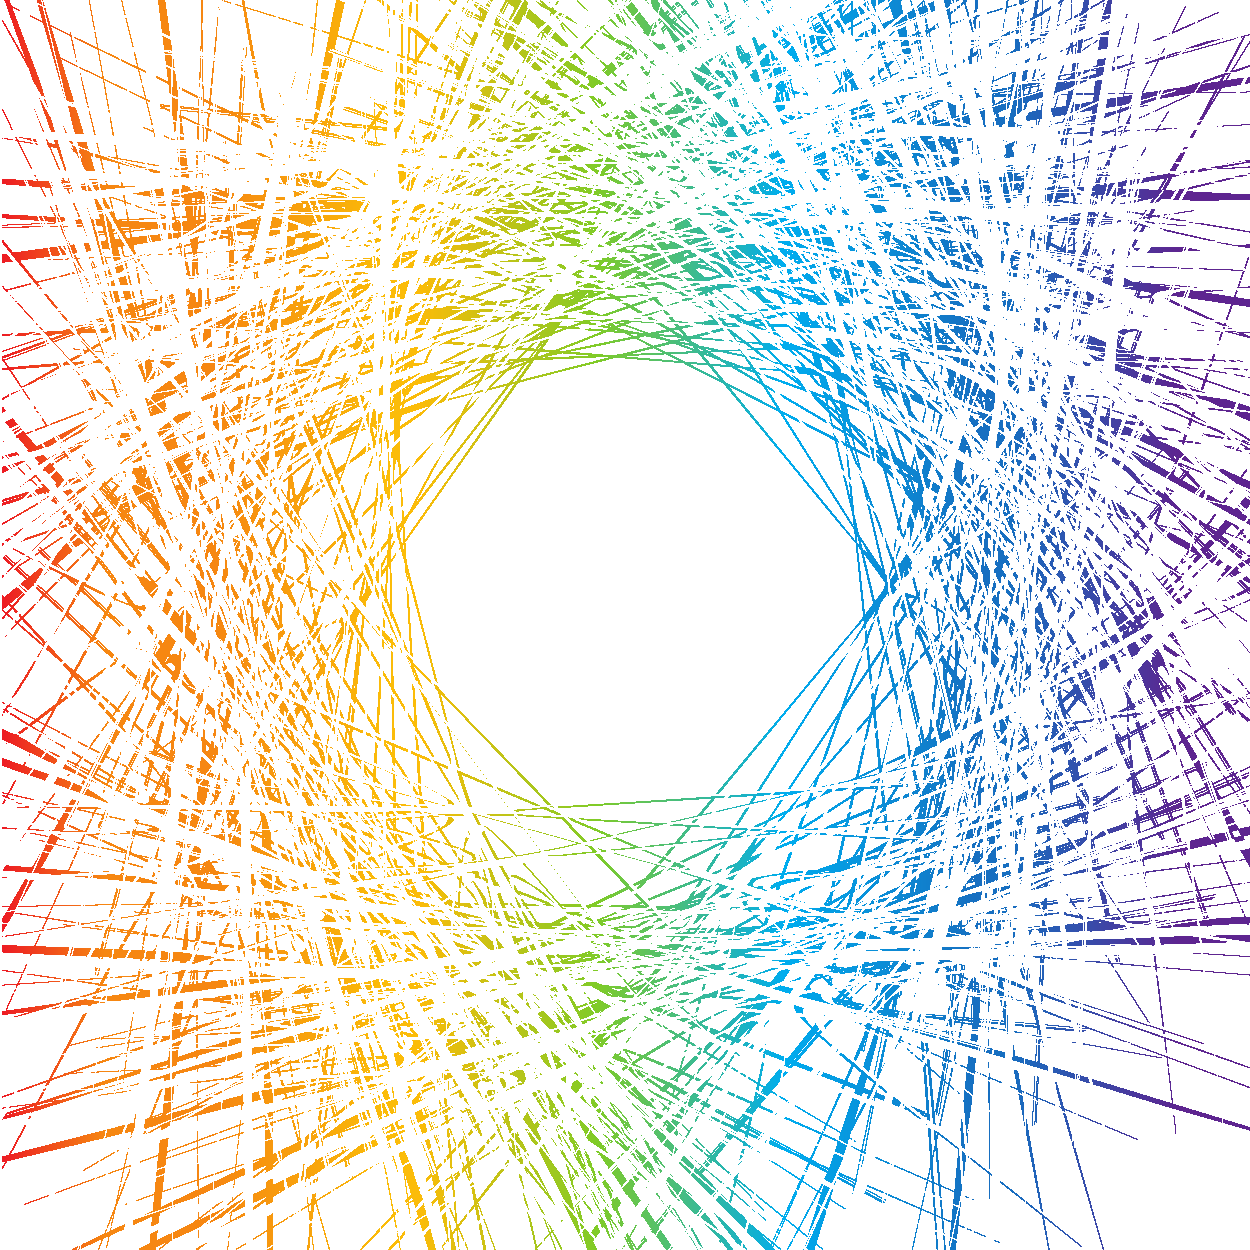
\includegraphics[width=\paperwidth,height=\paperheight]{img/Burst.pdf}
	}%
}


\begin{document}

\pagecolor{dark}
\color{white}
%\BgThispage
\sloppy
\centering
\vspace*{0.5em}
\begin{tabularx}{0.95\linewidth}{lR}
	\cref{white}{https://an7ar35.bitbucket.io/}{\raisebox{-0.4\height}{
\includegraphics[height=3em]{../common/graphics/avatar-whitespace.pdf}}\tab[0.5em] An7ar35} & 
	December 2017\newline \scriptsize{(Updated 02/01/18)}
\end{tabularx}

\vspace*{\fill}

\includegraphics[height=10em]{img/ArchMBP.pdf}\linebreak
\begin{mdframed}[style=titlebox]
	\centering
	\begin{Huge}
		\industrial{Arch Linux installation guide\linebreak
			for\linebreak
			MacBook Pro Retina mid 2015 model}\par
	\end{Huge}
\end{mdframed}
\vspace*{2em}

\includegraphics[height=5em]{img/kde-logo.pdf}with KDE\par
\vspace*{\fill}
\begin{tabularx}{0.95\textwidth}{lR}
	v1.0.1 & 
\includegraphics[height=3em]{../common/licenses/by-nc-sa_eu.pdf}
\end{tabularx}
\vspace*{2em}

\newgeometry{left=1cm,right=1cm,top=1cm,bottom=1.5cm}
\setcounter{page}{1}
\pagecolor{white}
\color{dark}
\normalsize\justify
\tableofcontents
\clearpage

\clearpage
\section{Foreword}

\begin{flushright}
	\textbf{This guide is current for the Linux kernel version \textcolor{red}{4.14.9-1}.}
\end{flushright}

\vspace*{1em}
After lots of reading, searching, experimenting, furious late-night shell command typing and do-overs here are the results of replacing OSX with Arch Linux on a mid-2015 MacBook Pro.

The setup is:
\begin{itemize}[noitemsep,topsep=0pt,leftmargin=*]
	\item Clean Arch installation, no OSX.
	\item Encrypted root/home/swap partition (luks),
	\item GRUB boot-loader (EFI),
	\item KDE Plasma desktop environment.
\end{itemize}

\vspace*{1em}
I would also advise backing up your drive using a complete bit-to-bit cloning process (unlike me who casually forgot that step... \begin{Large}\dejasans{😨}\end{Large}) so that you retain a copy of everything including the recovery partition on the Mac. This way it is a one-step process to restore everything.

This guide assumes a working knowledge of the Linux command line (bash) as well as Arch's \href{https://wiki.archlinux.org/index.php/Pacman}{\code{pacman}} and \href{https://archlinux.fr/yaourt-en}{\code{yaourt}\textsuperscript{AUR}} package managers.

\section{Nomenclature}

{\def\arraystretch{1.5}
\begin{tabularx}{\textwidth}{lX}
	\code{package-name} & Standard package \href{https://www.archlinux.org/packages/}{repository} - use \code{pacman} to install.\\
	\code{package-name}\textsuperscript{AUR} & Arch User Repository package (\href{https://aur.archlinux.org/}{AUR}) - use \code{yaourt} to install.\\
	\textcolor{orange}{\$} \code{...} & Command to type in at the command line prompt.\\
	\textcolor{codekeyword1}{\$TEXT} & User defined variable (replace with what you want to define it as).\\
	\key{Fn} & Function key.\\
	\key{⌃}  & Ctrl key.\\
	\key{⌥}  & Alt/Options key.\\
	\key{⌘}  & Command (Cmd) key.\\
	\key{⇧}  & Shift key.
\end{tabularx}
}

\clearpage
\section{Machine Specs}

\begin{tabularx}{\textwidth}{|c|X|}
	\hline
	Display   & \cbullet{15.4" LED-backlit Retina display (2880x1800 at 220ppi)} \\\hline
	Processor & \cbullet{2.5GHz quad-core Intel Core i7 processor (Turbo Boost up to 3.7GHz) with 6MB shared L3 cache} \\\hline
	RAM       & · 16GB of 1600MHz DDR3L memory \\\hline
	GPU       & · Intel Iris Pro Graphics, \newline
	· AMD Radeon R9 M370X with 2GB of GDDR5 memory\\\hline
	Storage   & · 512GB PCIe-based flash \\\hline
	Webcam    & · 720p FaceTime HD camera \\\hline
	Network   & · 802.11ac Wi‑Fi wireless networking; IEEE 802.11a/b/g/n compatible, \newline
	· Bluetooth 4.0 wireless technology \\
	\hline
\end{tabularx}

\section{Results}

\begin{small}\fcolorbox{linegrey}{white}{
		\textcolor{textgrey}{\textbf{Legend: }}
		\raisebox{-0.2\height}{\color{green}{\openiconic[]}} Works out-of-the-box or with few steps, 
		\raisebox{-0.2\height}{\color{blue}{\openiconic[]}} Requires some work, 
		\raisebox{-0.2\height}{\color{orange}{\openiconic[]}} Not fully working, 
		\raisebox{-0.2\height}{\color{red}{\openiconic[]}} Broken.}
\end{small}

\begin{center}
	{
	\def\arraystretch{1.2}
	\setlength\arrayrulewidth{1pt}
	\rowcolors{2}{gray!25}{white}
	\begin{tabularx}{\textwidth}{lcX}
		\rowcolor{white!50}
		\textbf{Item} & \textbf{Result} & \textbf{Note}\\
		\hline\hline
		Wifi\footnotemark[1] & \raisebox{-0.2\height}{\color{green}{\openiconic[]}} & Works out-of-the-box, some error messages.\\
		Bluetooth & \raisebox{-0.2\height}{\color{green}{\openiconic[]}} & Uses standard \code{bluez} package.\\
		Display (IPS scaling)\footnotemark[2] & \raisebox{-0.2\height}{\color{orange}{\openiconic[]}} & Mixed results without Wayland\\
		AMD Radeon R9 M370X & \raisebox{-0.2\height}{\color{blue}{\openiconic[]}} & Open source driver works like a charm,\newline screen brightness control requires \code{apple-gmux} to be patched\footnotemark[3].\\
		Intel Iris Pro Graphics\footnotemark[4] & \raisebox{-0.2\height}{\color{orange}{\openiconic[]}} & Disabled by default,\newline screen brightness control not working.\\
		Graphic switching & \raisebox{-0.2\height}{\color{orange}{\openiconic[]}} & Dynamic switching doesn't work.\newline Manual switching requires reboot and some TLC\footnotemark[5].\\
		Audio & \raisebox{-0.2\height}{\color{green}{\openiconic[]}} & Uses ALSA.\\
		FaceTimeHD camera\footnotemark[6] & \raisebox{-0.2\height}{\color{orange}{\openiconic[]}} & Requires firmware and driver from AUR. Suspend issues.\\
		Keyboard & \raisebox{-0.2\height}{\color{green}{\openiconic[]}} & ISO layout in command line but perfect in KDE.\\
		Keyboard (Backlight) & \raisebox{-0.2\height}{\color{green}{\openiconic[]}} & Works out-of-the-box.\\
		Keyboard \key{Fn} keys & \raisebox{-0.2\height}{\color{green}{\openiconic[]}} & Works out-of-the-box in KDE.
	\end{tabularx}
	}
\end{center}

\footnotetext[1]{Error messages with default kernel module but doesn't seem to affect connections.}
\footnotetext[2]{A workable solution can be setting the resolution to 1920x1200. The scale is good for a 15" screen.}
\footnotetext[3]{Patch needs to be re-applied after any kernel updates at the moment.}
\footnotetext[4]{When enabled, there are problems with back-lighting.}
\footnotetext[5]{Pain in the arse and not streamlined at all. Backlight control on Intel's IGU breaks.}
\footnotetext[6]{Not all applications seem to work with this camera but it might just be compatibility problems on the app side.}

\clearpage
\section{Pre-Installation}

\subsection{Preparations}

\textbf{Backup drive} (complete drive clone preferable).

Make a copy of the colour profile file(s) on the mac to a USB stick. It will be useful later on Linux. The profiles are located in \code{/Library/ColorSync/Profiles/Displays/*}.

\subsection{Making a bootable USB}

\subsubsection{From Linux}

\terminalcmd{dd if=archlinux.iso of=/dev/sdX bs=16M \&\& sync}
\block{Where \code{X} is your target USB drive letter (use \code{lsblk} for an overview of all connected drives to find out)}

\subsubsection{From a Mac}

\terminalcmd{diskutil unmountDisk diskX}
\block{Where \code{X} is your target USB drive number (use \code{diskutil list} for an overview of all connected drives to find out).}
\terminalcmd{sudo dd if=/Users/\$USERNAME/Downloads/archlinux.iso of=/dev/diskX bs=16M}
\block{Replace \textcolor{codekeyword1}{\$USERNAME} with your user-name on the mac and replace \code{X} with the USB drive's number.}

\section{Installation}

\subsection{Booting from the USB stick}

Simply plug in the USB in the MBP and press the \key{⌥} key during start up to reach the boot menu.

\subsection{Preliminary setup}

\terminalcmd{loadkeys uk}
\block{Load your keyboard layout. Replace `uk` with whichever you have on your machine.}
\terminalcmd{wifi-menu}
\block{Connect up to the wifi network. On the MPB Pro 2015 the wifi gets detected and works out of the box at this stage.}

\subsection{Partitioning and Crypto volume setup}

The assumption here is that the hard drive where everything will be installed to is \code{/dev/sda}. The partition structure will thus be: \\
\code{/dev/sda1} for the EFI partition,\\
\code{/dev/sda2} for the Boot partition and\\
\code{/dev/sda3} for the encrypted volume where the root, home and swap will be located.\\

\terminalcmd{cgdisk /dev/sda}
\begin{blocksection}
	\blockheader{Partition layout with just Linux}
	\textit{Warning: this will erase every thing including the recovery partition for OSX. \\
		No easy way to go back after this without a bit-to-bit HDD clone}
	\begin{enumerate}
		\item 100M partition `EFI' (Hex \#\code{ef00})
		\item 250M partition `Boot' (Hex \#\code{8300})
		\item 100\% remainder of the space for the crypto volume (Hex \#\code{8300})
	\end{enumerate}
	The root and home partition will be created later in the crypto volume
\end{blocksection}
\terminalcmd{cryptsetup --verbose --verify-passphrase --cipher aes-xts-plain64 --key-size 512 --hash sha512 --iter-time 5000 --use-random luksFormat /dev/sda3}
\block{Sets up the crypto volume.}
\terminalcmd{cryptsetup open --type luks /dev/sda3 mctoasty}
\block{\code{mctoasty} is the mounted name of the crypto volume. Can be changed to whatever is preferred.}

\subsubsection{Create crypto volume partitions}

\terminalcmd{pvcreate /dev/mapper/mctoasty}
\terminalcmd{vgcreate vg0 /dev/mapper/mctoasty}
\terminalcmd{lvcreate --size 16G vg0 --name swap}
\block{Generally swap size value is set to the amount of RAM.}
\terminalcmd{lvcreate --size 50GB vg0 --name root}
\block{Adjust root's size as required.}
\item \terminalcmd{lvcreate -l +100\%FREE vg0 --name home}
\block{Creates the home parition with the remainder of the free space.}

\subsubsection{Formatting all the partitions}

\terminalcmd{mkfs.vfat -F32 /dev/sda1}
\block{EFI partition}
\terminalcmd{mkfs.ext2 /dev/sda2}
\block{Boot partition}
\terminalcmd{mkswap /dev/mapper/vg0-swap}
\terminalcmd{mkfs.ext4 /dev/mapper/vg0-root}
\terminalcmd{mkfs.ext4 /dev/mapper/vg0-home}

\subsubsection{Mount all the partitions} \label{section:mount_all_the_partitions}

\terminalcmd{mount /dev/mapper/vg0-root /mnt}
\terminalcmd{swapon /dev/mapper/vg0-swap}
\terminalcmd{mkdir /mnt/boot}
\terminalcmd{mount /dev/sda2 /mnt/boot}
\terminalcmd{mkdir /mnt/boot/efi}
\terminalcmd{mount /dev/sda1 /mnt/boot/efi}
\terminalcmd{mkdir /mnt/home}
\terminalcmd{mount /dev/mapper/vg0-home /mnt/home}

\section{System Setup I: Base System Installation}

\terminalcmd{pacstrap /mnt base base-devel grub-efi-x86\_64 git efibootmgr bash-completion dialog wpa\_supplicant}
\begin{blocksection}
	Base packages along with GRUB and the EFI boot manager, git (will be useful later), bash completion and the stuff needed to keep the Wifi device in working order after reboot.
\end{blocksection}

\subsection{Generating fstab}

\terminalcmd{genfstab -pU /mnt >> /mnt/etc/fstab}
\begin{blocksection}
	\blockheader{Important!}
	This generates the fstab. i.e.: It saves our mounted partitions and swap configuration for persistence after a reboot. If you miss this step you'll have to reboot with the USB, mount everything again and then generate the fstab file.
\end{blocksection}
\terminalcmd{arch-chroot /mnt /bin/bash}

\subsection{System clock}

\terminalcmd{ln -s /usr/share/zoneinfo/\$ZONE/\$REGION /etc/localtime}
\begin{blocksection}
	Replace \textcolor{codekeyword1}{\$ZONE} with yours from \code{/usr/share/zoneinfo/}\\
	Replace \textcolor{codekeyword1}{\$REGION} with yours from \code{/usr/share/zoneinfo/\$ZONE/}\\
	e.g.: \code{/usr/share/zoneinfo/Europe/London}
\end{blocksection}
\terminalcmd{hwclock --systohc --utc}

\subsection{Hostname}

\terminalcmd{echo \$HOSTNAME > /etc/hostname}
\terminalcmd{nano /etc/hosts}
\begin{blocksection}
	Add the hostname at the end of each of the relevant lines in this file for completion's sake. Replace \textcolor{codekeyword1}{\$HOSTNAME} by the hostname you want to computer to have.
\end{blocksection}

\subsection{Basic fonts}

\terminalcmd{pacman -S terminus-font ttf-dejavu ttf-liberation}
\begin{blocksection}
	The terminus font will be used to make the console font more \href{https://wiki.archlinux.org/index.php/HiDPI#Linux_console}{readable} on the HiDPI display.
\end{blocksection}

\subsection{Locale}

\terminalcmd{locale-gen}
\block{Generates the locale file}
\terminalcmd{nano /etc/local.conf}
\block{Edit the locale configuration and delete the hash in front of the desired locale.}
\terminalcmd{local-gen}
\block{Needs to run again to apply the changes made in the previous step.}
\terminalcmd{nano /etc/locale.conf}
\begin{blocksection}
	To set permanent locale settings add the lines:
	\vspace*{1em}
	\begin{codeblock}
		LANG=en\_GB.UTF-8\\
		LANGUAGE=en\_GB\\
		LC\_ALL=C
	\end{codeblock}
\end{blocksection}

\subsection{Console keymap and font}

To see a list of all available keymaps: \code{find /usr/share/kbd/keymaps/ -type f | more}\\
To see a list of all installed console fonts: \code{ls /usr/share/kbd/consolefonts/}\\
For font maps check the \href{https://wiki.archlinux.org/index.php/fonts#Persistent_configuration}{Arch Wiki} and the \href{https://en.wikipedia.org/wiki/ISO/IEC_8859#The_parts_of_ISO/IEC_8859}{Wikipedia} entries.

\terminalcmd{nano /etc/vconsole.conf}
\begin{blocksection}
	To set permanent setting for the console add the lines:
	\vspace*{1em}
	\begin{codeblock}
		KEYMAP=uk\\
		FONT=ter-228n\\
		FONT\_MAP=8859-1
	\end{codeblock}
\end{blocksection}

\subsection{Root/User Accounts}

\terminalcmd{passwd}
\block{Sets the root password.}
\terminalcmd{useradd -m -g users -G wheel -s /bin/bash \$USERNAME}
\block{Adds a user. Replace \textcolor{codekeyword1}{\$USERNAME} with whatever user name you which to use.}
\terminalcmd{passwd \$USERNAME}
\block{Sets the user's password.}

\subsection{Initial RAM Environment Configuration [\href{https://wiki.archlinux.org/index.php/mkinitcpio}{\texttt{mkinitcpio}}]}

\terminalcmd{nano /etc/mkinitcpio.conf}
\begin{blocksection}
	In the file do the following:
	\begin{itemize}[noitemsep,topsep=0pt,leftmargin=*]
		\item In 'MODULES:
		\begin{enumerate}
			\item Add `ext4`
		\end{enumerate}
		\item In 'HOOKS':
		\begin{enumerate}
			\item Add \code{encrypt} and \code{lvm2} before \code{filesystems}
			\item Add \code{consolefont} right after \code{autodetect}\\
			(to avoid squinting at the crypto volume password prompt)
			\item Move \code{keyboard} right after \code{consolefont}
		\end{enumerate}
	\end{itemize}
	HOOKS should be ordered as such in the end:\\
	\code{HOOKS=(base udev autodetect consolefont keyboard modconf block encrypt lvm2 filesystems fsck)}
\end{blocksection}

\terminalcmd{mkinitcpio -p linux}
\block{Regenerates the initrd image.}

\subsection{GRUB boot loader}

\terminalcmd{grub-install}
\terminalcmd{nano /etc/default/grub}
\begin{blocksection}
	At line with \code{GRUB\_CMDLINE\_LINUX} add the arguments so that it becomes\\
	\code{GRUB\_CMDLINE\_LINUX="cryptdevice=/dev/sda3:luks:allow-discards"}
\end{blocksection}
\terminalcmd{grub-mkconfig -o /boot/grub/grub.cfg}

\subsection{Dismount and reboot}

\terminalcmd{umount -R /mnt}
\terminalcmd{swapoff -a}

Remove the USB stick then \code{reboot}.

\textbf{Note}: If you want a break (\begin{Large}\dejasans{☕}\end{Large}) this is the place to take it. Instead of rebooting just shutdown the machine.

\section{System Setup II: Hardware and Tools}

Reconnect to your wifi with \code{sudo wifi-menu}

\subsection{Enabling the multilib package repository}

\terminalcmd{nano /etc/pacman.conf}
\begin{blocksection}
	Uncomment the multilib lines (i.e. remove the leading \code{\#}):
	\vspace*{1em}
	\begin{codeblock}
		\#[multilib]\\
		\#Include = /etc/pacman.d/mirrorlist
	\end{codeblock}
\end{blocksection}
\terminalcmd{pacman -Syuu}
\block{Updates the cache/packages}

\subsection{AUR package manager - Yaourt}

There are two ways of doing this.

\vspace*{1em}
\textbf{\textcolor{textgrey}{\uline{a. Through Pacman}}}

\terminalcmd{sudo nano /etc/pacman.conf}
\begin{blocksection}
	Add the folowing lines to the end of the file:
	\vspace*{1em}
	\begin{codeblock}
		[archlinuxfr]\\
		SigLevel = Never\\
		Server = http://repo.archlinux.fr/\$arch
	\end{codeblock}
\end{blocksection}
\terminalcmd{sudo pacman -Syuu}
\terminalcmd{sudo pacman -S yaourt}

\vspace*{1em}
\textbf{\textcolor{textgrey}{\uline{b. Manual installation}}}

From your home directory (\code{cd \textasciitilde}):

\terminalcmd{mkdir -p git-repos/system-packages}
\terminalcmd{cd git-repos/system-packages}
\block{Or whatever directory chosen to clone the repositories into.}
\terminalcmd{git clone https://aur.archlinux.org/package-query.git}
\block{Required for \href{https://github.com/archlinuxfr/yaourt}{Yaourt}}
\terminalcmd{git clone https://aur.archlinux.org/yaourt.git}

For each of the 2 packages, \code{cd} into their respective directories and run the following command to install:

\terminalcmd{makepkg -si}
\block{e.g.: \code{cd package-query} then \code{makepkg -si}}

\vspace*{1em}
\textbf{\textcolor{textgrey}{\uline{Finally}}}
	
To build AUR packages with all 4 cores of the processor we need to modify the \code{makepkg.conf} file.

\terminalcmd{sudo nano /etc/makepkg.conf}
\begin{blocksection}
	Find the line:
	\begin{codeblock}
		\#MAKEFLAGS="-j2"		
	\end{codeblock}
	Uncomment the line and change the flag to \code{"-j4"}:
	\begin{codeblock}
		MAKEFLAGS="-j4"		
	\end{codeblock}
\end{blocksection}

\subsection{Console-Fu}

\terminalcmd{yaourt -S hstr-git}
\block{This is a replacement on \href{https://github.com/dvorka/hstr}{steroids} for the console's \key{⌃}+\key{R}}
\terminalcmd{hh --show-configuration >> \textasciitilde/.bashrc}
\block{Adds the config options for HSTR to your bash profile and auto-starts hh on login.}
\terminalcmd{pacman -S powertop htop}
\block{Installs 2 of the most basic and useful monitoring tools in linux.}

\subsection{Power management}

\terminalcmd{yaourt -S laptop-mode-tools}
\block{All the laptop-centric \href{https://wiki.archlinux.org/index.php/Laptop_Mode_Tools}{power saving} goodies}
\terminalcmd{sudo systemctl enable laptop-mode.service}
\block{Turns on the service} 
\terminalcmd{pacman -S acpid}
\block{\emph{(Optional)} \href{https://wiki.archlinux.org/index.php/Acpid}{Daemon} for delivering ACPI events.}

\subsection{Fans}

\terminalcmd{yaourt -S mbpfan-git}
	\block{\href{https://github.com/dgraziotin/mbpfan}{mbpfan-git}\textsuperscript{AUR} controls the MacBook's fans.}
\terminalcmd{sudo systemctl enable mbpfan.service}
	\block{Turns on the service}

The configuration file is located in \code{/etc/mbpfan.conf}. Go there to customise the temperature limits and fan speeds.

\subsection{Processor}

\terminalcmd{pacman -S intel-ucode}
\block{For intel's \href{https://wiki.archlinux.org/index.php/microcode}{microcode} update.}
\terminalcmd{grub-mkconfig -o /boot/grub/grub.cfg}
\block{Need to update grub so that it loads the Microcode updates at boot}

\subsubsection{Turbo Boost}

I would recommend disabling this feature if usage includes sustained load-heavy computation such as rendering, compiling, etc...

Turbo boost automatically increases the operating frequency of the cores depending on the task load. This allows for greater performance under demanding conditions but also causes heating issues. These are exasperated by the design constraint of laptops where large heat-sinks + fans or water-cooling is not practical.

Turning off Intel's CPU turbo boost makes a sizeable difference to temperature\footnote{Odly enough, I found that on my MBP the temperatures reached on OSX are a little worse than on Linux.} both on idle and under load. A cooler processor will also help increase the lifespan of the machine.

The table below shows the different temperature reached with and without the turbo boost enabled on my machine. The load was from compiling a small C++/Qt application.
The maximum turbo boost temperature was reached 10 seconds inside the compiling job and stayed at $100\,^{\circ}\mathrm{C}$ until completion with the fans going full blast.

\begin{center}
	\vspace*{1em}
	\rowcolors{2}{gray!25}{white}
	\setlength\arrayrulewidth{1pt}
	\begin{tabular}{|l|c|c|}
		\rowcolor{white!50}
		\hline
		\textbf{Turbo Boost state} & \textbf{Idle Temp.} & \textbf{Load Temp.}\\
		\hline\hline
		Enabled & $60\to 65\,^{\circ}\mathrm{C}$ & $100\,^{\circ}\mathrm{C}$\\ 
		Disabled &  $48\to 50\,^{\circ}\mathrm{C}$ & $76\,^{\circ}\mathrm{C}$\\
		\hline
	\end{tabular}
	\vspace*{1em}
\end{center}

\textbf{\textcolor{textgrey}{\uline{Requirements}}}

\href{https://01.org/msr-tools}{MSR-Tools}\textsuperscript{AUR} provides utilities to access the processor MSRs and CPU ID directly. It is called by the turbo-boost disabler script.

\terminalcmd{yaourt -S msr-tools}

\vspace*{1em}
\textbf{\textcolor{textgrey}{\uline{Disabling Turbo Boost}}}

Clone the \href{https://github.com/An7ar35/arch-scripts}{arch-scripts} repository into the \code{\textasciitilde/git-repos/system-packages} directory previously created.

\terminalcmd{cd \textasciitilde/git-repos/system-packages}
\terminalcmd{git clone https://github.com/An7ar35/arch-scripts}
\terminalcmd{cd arch-scripts/coreboost/}
\terminalcmd{sudo ./install.sh}
\begin{blocksection}
	The installation copies the \code{coreboost.sh} script into \code{/usr/local/bin/} and the systemd service file to launch that script into \code{/etc/systemd/system/}.\newline
	It then enables the service and loads it up. The turbo-boost disabler will be called upon at boot and after resuming suspend automatically.
\end{blocksection}

\subsection{Sound}

\href{https://wiki.archlinux.org/index.php/ALSA}{Alsa} works without issues.

\terminalcmd{sudo pacman -S alsa-utils alsa-plugins}
\terminalcmd{alsamixer}
\begin{blocksection}
	Make sure your current sound card is the "HDA Intel PCH" and that your master volume is up and unmuted (mute=MM, unmuted=00 at the bottom of the volume bar. You can use the \key{M} key on the keyboard to toggle mute).
\end{blocksection}
\terminalcmd{speaker-test -c 2}
\block{To make sure the sound works.}

\vspace*{1em}
\textbf{Note}: The internal speaker might not be disabled when using the headphone jack. To solve this, enable "Auto-mute" in \code{alsamixer}.

\subsection{Bluetooth}

\href{https://wiki.archlinux.org/index.php/Bluetooth}{Bluetooth} works out-of-the-box with the standard packages.

\terminalcmd{sudo pacman -S bluez bluez-utils}
\terminalcmd{modprobe btusb}
\terminalcmd{sudo systemctl enable bluetooth.service}

\subsection{Wifi}

\textbf{\textcolor{textgrey}{\uline{Broadcom Limited BCM43602 802.11ac Wireless LAN SoC (rev 01)}}}

As with most Broadcom chipsets, there are going to be hiccups. The \code{brcmfmac} driver is automatically loaded and works for the most parts (lucky!). Some have reported connectivity issues with this driver. Here is a run-down that includes my experience:

\vspace*{1em}
\begin{tabularx}{\textwidth}{cX}
	\raisebox{-0.2\height}{\color{green}{\openiconic[]}} & 2.4Ghz channels: works without issues.\\
	\raisebox{-0.2\height}{\color{orange}{\openiconic[]}} & 5Ghz channels: I haven't tested but both 2.4Hgz and 5Ghz capabilities are listed in \code{iw list}. \href{https://bugzilla.kernel.org/show_bug.cgi?id=193121}{Reports} say that they are not detected but that's for \textit{rev 2} of the chipset. - To be checked.\\
	\raisebox{-0.2\height}{\color{orange}{\openiconic[]}} & Low sensitivity: Lower than in OSX but not as bad as some reports.\\
	\raisebox{-0.2\height}{\color{green}{\openiconic[]}} & Failure after 10-15mns has not occurred in my case. Might be a \textit{rev 2} only issue.
\end{tabularx}

\subsection{Video}

\subsubsection{AMD Radeon}

Using the dedicated GPU means that the battery will drain faster than when using Intel's IGU but getting the backlight control to work has been relatively pain free.

\terminalcmd{sudo pacman -S mesa xf86-video-amdgpu vulkan-radeon lib32-mesa}
\begin{blocksection}
	Installs the open source drivers for the ATI GPU along with the 32bit libs and the Vulkan drivers.\\
	The \href{https://wiki.archlinux.org/index.php/Lm_sensors}{\code{lm\_sensors}} package used for temperature monitoring is a dependency for \code{mesa} so will be installed with it.\\
	Run \code{sensors} to see all the temperatures.
\end{blocksection}
\terminalcmd{yaourt -S radeontop}
\block{\emph{(Optional)} Monitoring utility for Radeon GPU cards.}

\subsubsection{Intel's IGU}

Getting Intel's IGU requires some work and is not perfect. First, the drivers:

\terminalcmd{sudo pacman -S xf86-video-intel}

\vspace*{1em}
\textbf{\textcolor{textgrey}{\uline{Enabling the Intel IGU}}}

We need to get the  \href{https://github.com/0xbb/apple\_set_os.efi}{apple\_set\_os.efi} binary from the repository's release section and unzip it. Then we need to copy it to the EFI partition:

\terminalcmd{sudo mkdir /boot/efi/EFI/custom}
\terminalcmd{sudo cp apple\_set\_os.efi /boot/efi/EFI/custom}

Then, \code{apple\_set\_os.efi} needs to be placed in GRUB's bootloader chain. I decided for a menu item in order to make triggering \code{apple\_set\_os.efi} optional.

\terminalcmd{lsblk --output MOUNTPOINT,LABEL,UUID}
	\block{Look for \code{/boot/efi} and \textbf{make a note of its UUID}.}
\terminalcmd{sudo nano /etc/grub.d/40\_custom}
\begin{blocksection}
	Add these lines to the file replacing \textcolor{codekeyword1}{\$UUID} with the UUID noted previously:\vspace*{1em}
	\begin{codeblock}
		menuentry \{\\
			\tab search --no-floppy --set=root --fs-uuid \textcolor{codekeyword1}{\$UUID}\\
			\tab chainloader (\$\{root\})/EFI/custom/apple\_set\_os.efi\\
		\}
	\end{codeblock}
\end{blocksection}
\terminalcmd{sudo grub-mkconfig -o /boot/grub/grub.cfg}
	\block{Updates GRUB with the changes.}

\subsubsection{Switching GPUs}

This section assumes both the AMD and Intel installations have been done. An extra package (\href{https://github.com/0xbb/gpu-switch}{gpu-switch\textsuperscript{AUR}}) is required to be able to switch between the integrated and dedicated GPUs on the MBP 11,5.

\terminalcmd{yaourt -S gpu-switch}

\vspace*{1em}
\textbf{\textcolor{textgrey}{\uline{Switching to the integrated GPU (\raisebox{-0.2\height}{
\includegraphics[height=1.2em]{img/Intel-logo.pdf}}):}}}

\terminalcmd{sudo gpu-switch -i}

Then use the "\textit{apple\_set\_os}" menu option in GRUB at boot before your normal "\textit{Arch}" menu option.

\vspace*{1em}
\textbf{\textcolor{textgrey}{\uline{Switching to the dedicated GPU (\raisebox{-0.2\height}{
\includegraphics[height=1.2em]{img/ATI_logo.pdf}}):}}}

\terminalcmd{sudo gpu-switch -d}

Then \textbf{only} use your normal "\textit{Arch}" menu option in GRUB at boot (default).

\subsubsection{Display brightness}

\textbf{Note}: this only applies to the AMD Radeon. Brightness control currently does not work on the Intel IGU aside from turning it either on/off completely.

To get brightness control to work, a patched version of the \code{apple-gmux} kernel module is required. The vanilla module does \href{https://bugzilla.kernel.org/show_bug.cgi?id=105051#c37}{not work} for the current Linux kernel. Perhaps later versions will eventually.

An easy installer script is available in the \href{https://github.com/An7ar35/arch-scripts}{arch-script repository}.

If you haven't previously cloned the repository (Turbo Boost section):

\terminalcmd{cd \textasciitilde/git-repos/system-packages}
\terminalcmd{git clone https://github.com/An7ar35/arch-scripts}

\vspace*{1em}
\textbf{\textcolor{textgrey}{\uline{Installing the patched module}}}

\terminalcmd{cd arch-scripts/mbp-brightness-patch/}
\terminalcmd{sudo ./install.sh}

Then restart the machine.

\vspace*{1em}
\textbf{\textcolor{textgrey}{\uline{Kernel updates}}}

If the brightness control breaks after a kernel update the patch installer must be run again to get the functionality back.

\subsection{Keyboard}

All of these tweaks are optional and based on personal choice. The one's I have not tested are marked as such.

\vspace*{1em}
\textbf{\textcolor{textgrey}{\uline{Switch function keys on by default}}}

To make function keys be used as first keys. i.e.: Pressing \key{F1} key alone will behave like F1 and pressing \key{Fn}+\key{F1} will act as the special key (brightness down).

\terminalcmd{sudo nano /etc/modprobe.d/hid\_apple.conf}
\begin{blocksection}
	Add the following line to the file:
	\vspace*{1em}
	\begin{codeblock}
		options hid\_apple fnmode=2
	\end{codeblock}
\end{blocksection}
\terminalcmd{sudo mkinitcpio -p linux}
	\block{Updates the \textit{initramfs} with the new configuration.}

\vspace*{1em}
\textbf{\textcolor{textgrey}{\uline{Swap the} \key{⌥} \uline{and} \key{⌘} \uline{keys (untested)}}}

\terminalcmd{sudo nano /etc/modprobe.d/hid\_apple.conf}
\begin{blocksection}
	Add the following line to the file:
	\vspace*{1em}
	\begin{codeblock}
		options hid\_apple swap\_opt\_cmd=1
	\end{codeblock}
\end{blocksection}
\terminalcmd{sudo mkinitcpio -p linux}
\block{Updates the \textit{initramfs} with the new configuration.}

\subsection{Webcam}

The 2015 MBP has \href{https://wiki.archlinux.org/index.php/MacBook#Facetime_HD}{Facetime HD}.
Fortunately there is a \href{https://github.com/patjak/bcwc_pcie}{reversed-engineered driver} but "PC suspension is not supported if a 
program that is keeping the camera active is running".

To make it work, first install the firmware then the driver from AUR:

\terminalcmd{yaourt -S facetimehd-firmware}
\terminalcmd{yaourt -S bcwc-pcie-git}

To test the webcam, \code{mplayer tv://} or the \lq \textit{Qt 4VL Test Utility}\rq\ can be used inside KDE.

\begin{table}[!h]
	\centering
	\vspace*{1em}
	\rowcolors{2}{gray!25}{white}
	\setlength\arrayrulewidth{1pt}
	\caption*{Tested applications} \label{tab:tested-webcam-apps} 
	\begin{tabular}{|l|l|c|}
		\rowcolor{white!50}
		\hline
		\textbf{App} & \textbf{Version} & \textbf{Works?} \\
		\hline\hline
		Discord & 0.0.3-1 & \ding{51}\\
		Skype & 8.13.76.6-1 & \ding{55}\\
		Kamoso & 3.2.4-1 & \ding{55}\\
		\hline
	\end{tabular}
	\vspace*{1em}
\end{table}

\subsection{Touchpad}

Basic touchpad support is available with the Linux kernel. If you want to customise your experience, a specialised synaptic driver must be installed. There are 3 options to choose from. Make sure you only have one installed at any one time to avoid conflicts.

\vspace*{1em}
\textbf{\textcolor{textgrey}{\uline{Option 1: \href{https://wiki.archlinux.org/index.php/Libinput}{\code{libinput}}}}}

\terminalcmd{sudo pacman -S libinput}

To add gestures, the  \href{https://github.com/bulletmark/libinput-gestures}{\code{libinput-gestures}\textsuperscript{AUR}} package can be installed:

\terminalcmd{yaourt -S libinput-gestures}
\terminalcmd{sudo gpasswd -a \$USERNAME imput}
	\begin{blocksection}
		Adds \textcolor{codekeyword1}{\$USERNAME} to the \lq input\rq\ group.
	\end{blocksection}
\terminalcmd{libinput-gesture-setup autostart}

The Arch Wiki states that there may be an \href{https://wiki.archlinux.org/index.php/Libinput#Touchpad_settings_not_taking_effect_in_KDE.27s_Touchpad_KCM}{issue} where settings do not take effect from the KDE vanilla \lq\textit{System Settings}\rq\ touchpad panel. 

Optionally, a \href{https://github.com/amezin/pointing-devices-kcm}{rewritten KCM} for all for all input devices supported by \code{libinput} is available from the  \href{https://aur.archlinux.org/packages/kcm-pointing-devices-git/}{AUR repository}:

\terminalcmd{yaourt -S kcm-pointing-devices-git}

\vspace*{1em}
\textbf{\textcolor{textgrey}{\uline{Option 2: \code{xf86-input-synaptics}}}}

The standard synaptic driver. KDE will detect it and enable you to change its settings within the \lq System Settings\rq\ panel. Only supports 2 finger gesture though.

\terminalcmd{sudo pacman -S xf86-input-synaptics}

\vspace*{1em}
\textbf{\textcolor{textgrey}{\uline{Option 3: \code{xf86-input-mtrack}\textsuperscript{AUR}}}}

Multi-touch support but KDE does \textbf{not} natively detect it so settings must be set manually in \code{/etc/X11/xorg.conf.d/10-mtrack.conf}. A full list of supported options is available in the project's Github \href{https://github.com/p2rkw/xf86-input-mtrack}{repository}.

\terminalcmd{yaourt -S xf86-input-mtrack}

\subsection{Other Drivers}

Possible missing firmware module for:
\begin{itemize}[noitemsep,topsep=0pt,leftmargin=*]
	\item wd719x
	\item aic94xx
\end{itemize}

\terminalcmd{pacman -S aic94xx-firmware}
\terminalcmd{pacman -S wd719x-firmware}
\terminalcmd{sudo mkinitcpio -p linux}
\block{To make sure drivers are loaded.}

\section{System Setup III: Desktop}

Wayland support as of Dec 2017 on KDE is beta at best. Scaling in nice but buggy as hell displaying artefacts. Until that gets a lot better Xorg is the default choice as display managers go even if HiDPI support is terrible. 

\subsection{Display server (\href{https://wiki.archlinux.org/index.php/xorg}{Xorg})}

\terminalcmd{sudo pacman -S xorg, xorg-server xorg-xinit}

\subsection{Desktop Environment (\href{https://wiki.archlinux.org/index.php/KDE}{KDE})}

A display manager (\href{https://wiki.archlinux.org/index.php/SDDM}{SDDM}) is installed along with KDE to make it easy to automatically run KDE when starting a user session and provide a GUI login too.

\terminalcmd{sudo pacman -S plasma kde-applications sddm systemd-kcm}
\terminalcmd{sudo systemctl enable sddm.service}
\terminalcmd{sudo systemctl start sddm.service}

Auto-login can be configured inside KDE's \lq System Settings\rq\ panel (\lq Startup \& Shutdown\rq\ \rightarrow\ \lq Login Screen (SDDM)\rq\ \rightarrow\ \lq Advanced\rq\ tab).

\terminalcmd{sudo pacman -S xdg-user-dirs}
\begin{blocksection}
	\blockheader{Optional} 
	Create all the default \href{https://wiki.archlinux.org/index.php/XDG_user_directories}{user directories} such as \lq Downloads\rq\ , \lq Music\rq\  , etc...
\end{blocksection}

\subsection{Network manager (Wifi)}
\terminalcmd{sudo systemctl enable NetworkManager.service}
\block{Enables the network service. GUI network connections should work after reboot.}

\subsection{GUI package manager}

\href{https://wiki.manjaro.org/index.php?title=Pamac}{Pamac} is a nice package manager with AUR support. It can be installed with:

\terminalcmd{yaourt -S pamac-aur}
\block{AUR support can be explicitly enabled inside the application's settings in the AUR tab.}

\subsection{Colour Profile}

To use the previously saved OSX colour profile(s) copy them/it to your home directory under \code{.color/icc/}. 

If you don't plan on using KDE and/or want an agnostic way of loading colour profiles then install \code{xcalib}\textsuperscript{AUR} and follow the instructions provided in the \href{https://wiki.archlinux.org/index.php/mac#Color_Profile}{Arch Wiki}.

\textbf{\textcolor{textgrey}{\uline{For KDE}}}

\terminalcmd{sudo pacman -S colord-kde}
\begin{blocksection}
	Then, in \lq Systems Settings\rq\ under the \lq Color Corrections\rq\ section, add your profile file wanted to the \lq\textit{Apple - MacBookPro11,5}\rq\ and tick it instead of the pre-given default.
\end{blocksection}

\subsection{Peripherals}

These are generic package installations required to make most printers and scanners work. Additional steps may (very likely!) be required to get these peripherals working in Linux.

\subsubsection{Printing}

\terminalcmd{sudo pacman -S cups print-manager}

\subsubsection{Scanning}

\terminalcmd{sudo pacman -S sane libksane sane-frontends xsane}
\terminalcmd{sudo pacman -S skanlite}
	\block{Simple image scanning application for KDE.}

\vspace*{1em}
If you have an Epson scanner:

\terminalcmd{sudo pacman -S iscan iscan-data}

\section{System Setup IV: Applications}

\subsection{File system}

\terminalcmd{sudo pacman -S ntfs-3g exfat-utils}
\block{Enables access to NTFS and ExFAT file systems.}
\terminalcmd{sudo pacman -S gparted}
\block{Partition manager. Alternatively there is also \code{partitionmanager} (KDE)}

\subsection{Firewall}

Install \code{firewalld} and start the \code{firewalld.service}

If there is a systemd timeout \href{https://bugzilla.redhat.com/show_bug.cgi?id=1294415#c10}{issue} on restart, do:

\terminalcmd{sudo nano /etc/firewalld/firewalld.conf}
\begin{blocksection}
	Find the \code{CleanupOnExit} option in the file and set it to `\code{no}':
	\vspace*{1em}
	\begin{codeblock}
		CleanupOnExit=no
	\end{codeblock}
\end{blocksection}

\subsection{Compression, Archiving and Backup}

\begin{varwidth}[t]{.5\textwidth}
\textbf{\textcolor{textgrey}{\uline{Terminal}}}
	\begin{itemize}[noitemsep,topsep=0pt,leftmargin=*]
		\item \code{p7zip}
		\item \code{unrar}
		\item \code{zip}
		\item \code{unzip}
	\end{itemize}
\end{varwidth}
\hspace{4em}
\begin{varwidth}[t]{.5\textwidth}
	\textbf{\textcolor{textgrey}{\uline{GUI}}}
	\begin{itemize}[noitemsep,topsep=0pt,leftmargin=*]
		\item \code{ark} (Compression)
		\item \code{deja-dup} (Backup)
	\end{itemize}
\end{varwidth}

\subsection{Dolphin extras}

\terminalcmd{sudo pacman -S kde-thumbnailer-odf kde-thumbnailer-epub kde-thumbnailer-gimpsources}
\block{Adds thumbnail support to ODF, EPUB and gimp source files. Enable in Dolphin's settings.}

\subsection{Fonts}

Some more fonts for the system. If more are required, a good place to find some is the \href{https://fontlibrary.org/}{Font Library} which has a large collection of fonts with permissive licenses.

\begin{varwidth}[t]{.5\textwidth}
	\begin{itemize}[noitemsep,topsep=0pt,leftmargin=*]
		\item \code{adobe-source-code-pro}
		\item \code{adobe-source-sans-pro}
		\item \code{adobe-source-serif-pro}
	\end{itemize}
\end{varwidth}
\hspace{4em}
\begin{varwidth}[t]{.5\textwidth}
	\begin{itemize}[noitemsep,topsep=0pt,leftmargin=*]
		\item \code{ttf-mac-fonts}\textsuperscript{AUR}
	\end{itemize}
\end{varwidth}

\subsection{Nice extra packages}

\begin{center}
	{
		\def\arraystretch{1.2}
		\setlength\arrayrulewidth{1pt}
		\rowcolors{2}{gray!25}{white}
		\begin{tabularx}{\textwidth}{XcX}
			\rowcolor{white}
			\textbf{Package} & \textbf{Environment} & \textbf{Description}\\
			\hline\hline
			\code{cmus} & Term & Nice little console \href{https://cmus.github.io/}{music player}.\\
			\code{wget} & Term & Command line \href{https://www.gnu.org/software/wget/}{tool} to retrieve files using HTTP, HTTPS, FTP and FTPS.\\
			\code{yakuake} & KDE & Quake-like tidle \href{https://yakuake.kde.org/}{console}.\\
			\code{cairo-dock}\linebreak \code{cairo-dock-plugins} & GUI & \href{https://www.glx-dock.org/}{Docks} like on a mac.\\
			\code{redshift}\linebreak \code{plasma5-applets-redshift-control} & GUI/KDE & Colour temperature \href{http://jonls.dk/redshift/}{adjuster} and KDE controller applet.\\
			\code{firefox} & GUI & Web browser.\\
			\code{thunderbird} & GUI & Mail client.
		\end{tabularx}
	}
\end{center}

\clearpage
\section{Troubleshooting}

\subsection{Kernel errors}
\subsubsection{USB suspend error}

If you get the following sort of error after suspend/sleep:
\vspace*{0.6em}
\begin{codeblock}
	usb 2-4: usb\_reset\_and\_verify\_device Failed to disable LTM\linebreak	
	usb usb2-port4: cannot disable (err=-32)
\end{codeblock}

The Kernel \href{https://bugzilla.kernel.org/show_bug.cgi?id=117811}{Bug report \#117811}'s thread suggest disabling USB auto-suspend.

\begin{itemize}[noitemsep,topsep=0pt,leftmargin=*]
	\item If you are using \href{https://wiki.archlinux.org/index.php/TLP}{TLP}:\\
	\code{nano /etc/default/tlp} and set \code{USB\_AUTOSUSPEND=0}
	\item If you are \textbf{not} using \href{https://wiki.archlinux.org/index.php/TLP}{TLP}:\\
	\code{sudo echo on | tee /sys/bus/usb/devices/*/power/control}
\end{itemize}

\subsection{Boot partition recognition is slow}

This is usually caused by booting a OSX drive externally or creating one with the recovery process (started with with \key{⌘}+\key{R} on the MacBook Pro). 

\textbf{Beware:} Before going forward, make sure you have an \underline{bootable Arch installation USB drive} ready as you will also need to go reinstall GRUB as described in the next section.

To remedy this problem you will need to \href{https://support.apple.com/en-us/HT204063}{reset the NVRAM} by pressing \key{⌥}+\key{⌘}+\key{P}+\key{R} together and turn on the machine keeping them pressed for about 20 seconds (or until the second boot-up chime).

\subsection{Boot partition not detected after NVRAM reset}

Boot from the Arch setup USB (see section `Making a bootable USB').

Mount all the partitions again (see section \ref{section:mount_all_the_partitions}) without making the directories:

\terminalcmd{mount /dev/mapper/vg0-root /mnt}
\terminalcmd{mount /dev/mapper/vg0-home /mnt/home}
\terminalcmd{mount /dev/sda2 /mnt/boot}
\terminalcmd{mount /dev/sda1 /mnt/boot/efi}
\terminalcmd{swapon /dev/mapper/vg0-swap}

Get into the \code{arch-chroot} environment and reinstall GRUB:

\terminalcmd{arch-chroot /mnt /bin/bash}
\terminalcmd{run mkinitcpio -p linux}
\terminalcmd{run grub-install}
\terminalcmd{grub-mkconfig -o /boot/grub/grub.cfg}

Exit chroot environment and shutdown:

\terminalcmd{exit}
\terminalcmd{shutdown now}

Remove the USB stick and boot up.

\subsection{Text-to-Speech isn't working}

Check \code{journalctl -b} for an error relating to \code{flite} being missing. Installing it should resolve the text-to-speech problem.

\terminalcmd{sudo pacman -S flite}

\clearpage
\section{References}

\begin{itemize}
	\item \href{https://wiki.archlinux.org/index.php/MacBookPro11,x#Using_the_MacBook.27s_native_EFI_bootloader_.28recommended.29}{Arch Linux's MacBookPro 11.x Wiki page}
	\item \href{https://gist.github.com/mattiaslundberg/8620837}{Mattias Lindberg's Encrypted volume Arch install guide}
	\item \href{https://www.howtoforge.com/tutorial/how-to-install-arch-linux-with-full-disk-encryption/}{HowToForge | How to install Arch Linux with Full Disk Encryption}
	\item \href{https://help.ubuntu.com/community/AppleKeyboard#Change_Function_Key_behavior}{Ubuntu | AppleKeyboard}
\end{itemize}

\end{document}
